\section{Application Description}
\subsection{Research related applications/systems}
The selected reference application is \textbf{Shopee}, one of the leading E-Commerce platforms in Vietnam. The website can be accessed at \href{https://shopee.vn}{https://shopee.vn}. \textbf{Shopee} connects customers and sellers in an online marketplace, providing a comprehensive system to browse, purchase, and manage products. Its business process begins with account registration, where users can sign up as customers or sellers. Customers browse products organized in hierarchical categories, select variants of products such as size or color, add items to a shopping cart, and proceed to checkout with payment and shipping options. Sellers manage shop profiles, upload and update product listings, track inventory, and monitor customer reviews to improve service quality.\\

A key feature of \textbf{Shopee} is the multi-shop order system, where a single order can include products from multiple sellers, each tracked individually in the backend. Another important element is the voucher system, which applies discounts based on conditions such as minimum order value or expiration dates. \textbf{Shopee} also integrates a review and rating system, ensuring that verified purchases can leave feedback on the product and the store, which helps improve trust and transparency.\\

\begin{figure}[H]
    \centering
    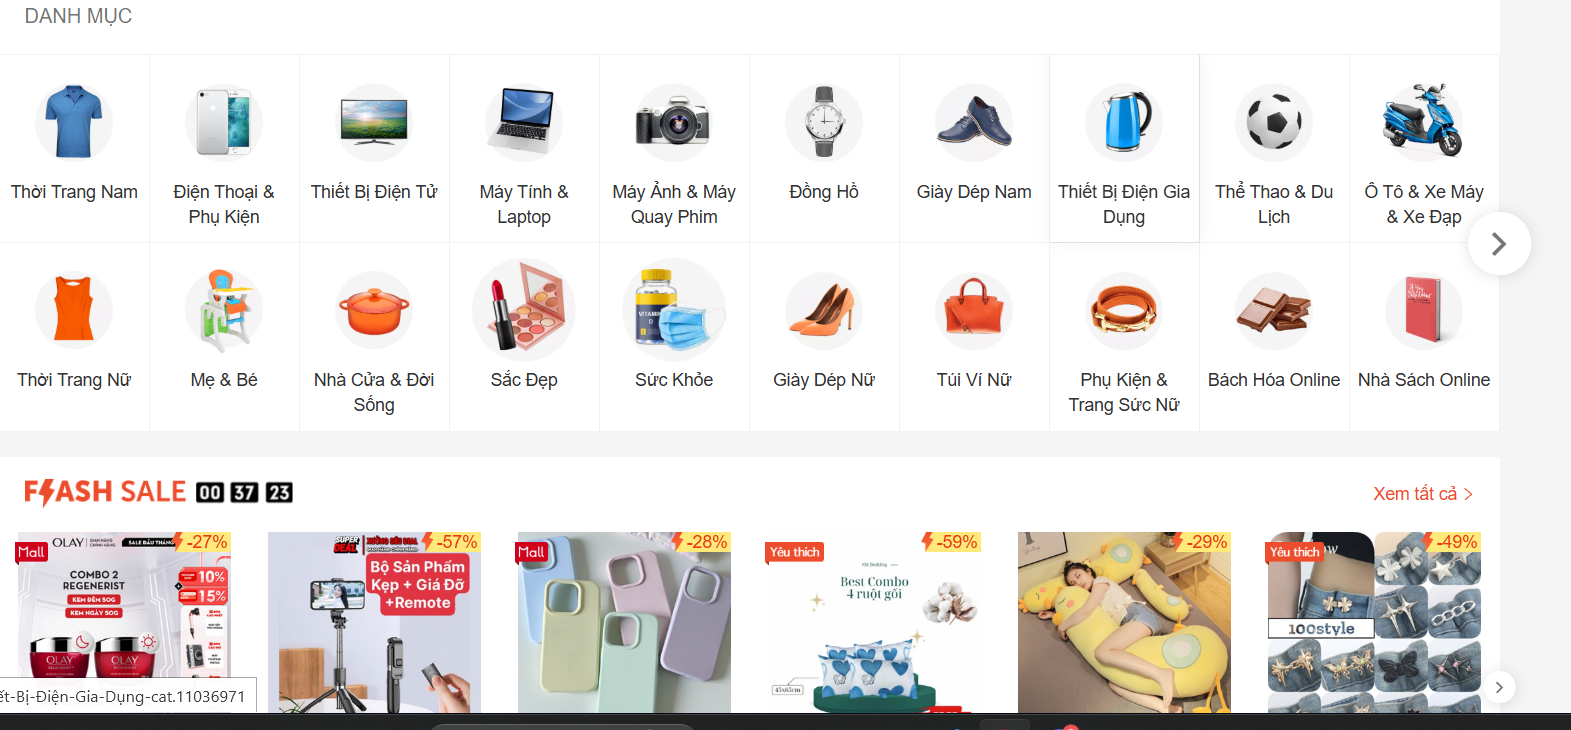
\includegraphics[width=0.8\textwidth]{img/shoppee2.png}
    \caption{Homepage interface of \textbf{Shopee} when accessing the website for the first time}
\end{figure}

\noindent
The homepage highlights featured campaigns, recommended products, and navigation menus, such as categories, products and flash sales. This layout indicates that \textbf{Shopee} focuses heavily on visual-driven marketing and personalized product discovery.

\begin{figure}[H]
    \centering
    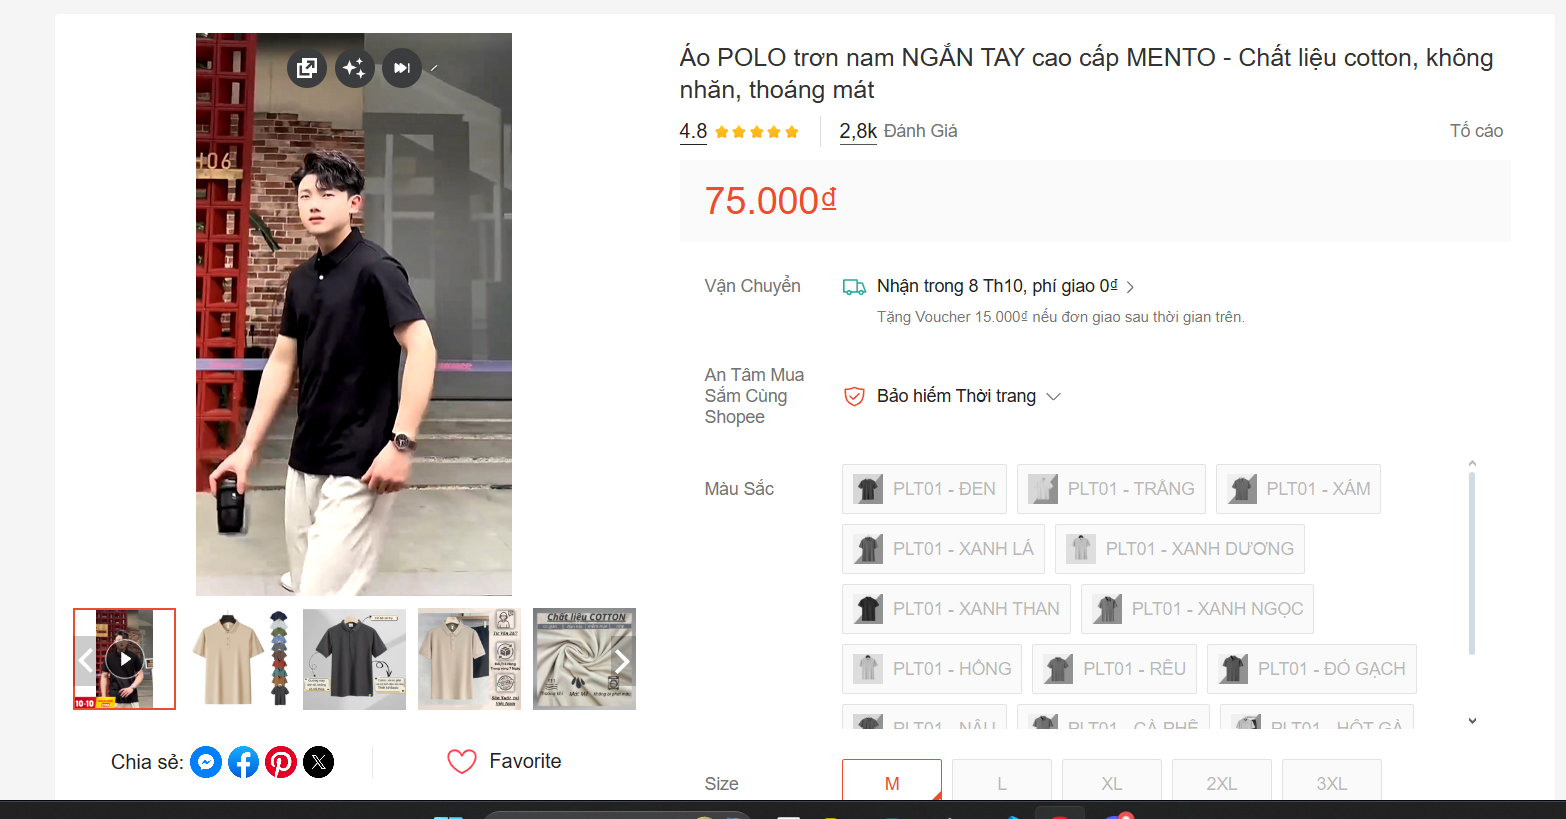
\includegraphics[width=0.8\textwidth]{img/shoppee1.png}
    \caption{Product detail page with variant selection (size, color), price display, and image gallery}
\end{figure}

\noindent
This screen demonstrates the purchasing flow, where users can select a specific \textbf{product variant}, adjust quantity, add to cart or directly place an order. Essential information such as ratings, shipping options, and shop reputation is also displayed to support decision-making.

\subsection{Description of the Proposed System}

\subsubsection{General Description}

The proposed system is an e-commerce platform inspired by Shopee, designed to support online retail activities between buyers and sellers. It enables individuals and businesses to create selling accounts, publish products, and manage orders, while customers can browse, purchase, and evaluate products in a seamless digital marketplace.

\paragraph{Types of Users:}

\textbf{Customer}: A regular user who browses products, adds items to their shopping cart, places orders, applies vouchers, selects shipping methods, and provides product or shop reviews after successful purchases.

\textbf{Shop}: A seller entity responsible for managing product listings, defining product variants, monitoring stock levels, handling orders, and receiving feedback from customers.

\textbf{Admin}: A privileged system user who supervises overall platform operations, manages user accounts, resolves disputes, and moderates inappropriate content when necessary.
\paragraph{Main System Functions:}

For \textbf{Customers}: Browse products by category, search and filter based on attributes, add items to cart, update quantities, place orders with preferred shipping and payment methods, apply vouchers, and submit verified reviews for purchased products.

For \textbf{Shops}: Register as sellers, manage store profile, create product listings with multiple variants, track inventory, process incoming orders, and analyze ratings and feedback to improve service quality.

For \textbf{Admins}: Oversee account registration activities, suspend violating accounts, manage system-wide configurations such as shipping options and voucher policies, and intervene in reported cases of fraud or misconduct.

\subsubsection{Detailed Description of Entity Types, Attributes and Relationships}

\paragraph{ACCOUNT Entity}

The system maintains a centralized \textbf{ACCOUNT} entity to identify every registered user. Each account is uniquely defined by an \textbf{AccountID} (auto-incremented primary key) and stores essential authentication details such as \textbf{Email} and \textbf{Password}. Personal identification is represented through the attribute \textbf{FullName}, while \textbf{Phone} stores the primary contact information and must follow Vietnamese phone format (10 digits). The \textbf{Role} field classifies each account as Customer, Shop, or Admin, ensuring proper access control. The attribute \textbf{Status} maintains activation state with values `Active' or `Ban' for moderation purposes. \textbf{CreatedAt} records the registration timestamp automatically.

\paragraph{CUSTOMER Entity}

The \textbf{CUSTOMER} entity is a specialization of ACCOUNT and represents end-users participating in purchasing activities. Each customer is referenced by a distinct \textbf{CustomerID} (same as AccountID) and an auto-generated \textbf{CustomerCode} with `CUST' prefix (CUST00001, CUST00002, ...). Customers have an \textbf{Address} for default shipping destination and \textbf{AddPhone} for additional contact. The system maintains \textbf{TotalSpent} and \textbf{TotalOrder} as derived attributes to support customer ranking and loyalty programs. Each CUSTOMER owns exactly one \textbf{CART}.

\paragraph{SHOP Entity}

The \textbf{SHOP} entity models registered merchants. Each shop is assigned a unique \textbf{ShopID} (same as AccountID) and an auto-generated \textbf{ShopCode} with `SHOP' prefix (SHOP00001, SHOP00002, ...). A shop operates under a \textbf{ShopName} and has a \textbf{ShopPhone} for business inquiries. The \textbf{AddressShop} identifies its operational base, while \textbf{Rating} reflects aggregated customer feedback (0-5 scale). The \textbf{ShopStatus} attribute can be `Open', `Temporarily Close', or `Closed'. A single SHOP may publish multiple \textbf{PRODUCTS}.

\paragraph{ADMIN Entity}

The \textbf{ADMIN} entity represents internal supervisory staff. Each admin is identified by an \textbf{AdminID} (same as AccountID) and is linked to an \textbf{AccountID}. The \textbf{Role} field specifies the admin's level of access (Core, Moderator, or Support), ensuring proper authorization. Unlike other roles, admins do not engage in transactions but retain full access rights for system governance. \textbf{Note} field allows additional admin information.

\paragraph{CATEGORY Entity}
The \textbf{CATEGORY} entity organizes products into a navigable structure. Each category has a unique \textbf{CategoryID} and a descriptive \textbf{CategoryName} (max 100 characters). Categories support hierarchical organization through \textbf{ParentCategoryID}, which can be null for root categories. This recursive 1:N relationship enables multi-level product browsing.

\paragraph{PRODUCT Entity}

The \textbf{PRODUCT} entity represents commercial goods listed by shops. Each product is uniquely defined by a \textbf{ProductID}, belongs to exactly one SHOP through \textbf{ShopID}, and must be classified under a CATEGORY via \textbf{CategoryID}. Descriptive attributes include \textbf{ProductName}, \textbf{Description}, \textbf{Image}, and \textbf{CreatedAt}. The attribute \textbf{Status} specifies whether the product is `In stock' or `Out of stock'. \textbf{Rating} is auto-calculated from customer reviews. Products serve as parent entities for \textbf{PRODUCTITEM} (variants).

\paragraph{PRODUCTITEM Entity}

\textbf{PRODUCTITEM} is a weak entity that models purchasable variations of a product. Each item is uniquely identified by \textbf{ItemID} and belongs to a specific \textbf{ProductID}. Each variant contains attributes such as \textbf{Color}, \textbf{Type} (size, configuration), \textbf{Price}, \textbf{Stock}, and optionally \textbf{ImageURL} for representation. Variants enable customers to differentiate between sizes, configurations, or styles within the same product family. \textbf{ShopID} is stored for quick reference to the selling shop.

\paragraph{CART Entity}

The \textbf{CART} entity holds temporary selections before checkout. Each cart is exclusively owned by one CUSTOMER and distinguished by \textbf{CartID}. The relationship between CART and PRODUCTITEM is modeled as a many-to-many association through \textbf{CARTITEM}, enriched with the attribute \textbf{Quantity}. \textbf{CreatedAt} and \textbf{UpdatedAt} track cart lifecycle.

\paragraph{CARTITEM Entity}

\textbf{CARTITEM} is a junction table representing the many-to-many relationship between CART and PRODUCTITEM. Each entry is identified by \textbf{CartItemID} and contains \textbf{Quantity} (the number of units chosen for each specific variant).

\paragraph{ORDER Entity}
The \textbf{ORDER} entity records finalized purchases. Each order is uniquely identified by an \textbf{OrderID} and linked to a CUSTOMER via \textbf{CustomerID}. Transaction attributes include \textbf{OrderDate}, \textbf{ShippingAddress}, and \textbf{PaymentMethod} (COD, Banking, Momo, ZaloPay). The system computes \textbf{TotalAmount} automatically based on selected variants and applied promotions. Each order references exactly one \textbf{SHIPPING} through \textbf{ShippingID} and may optionally apply a \textbf{VOUCHER} through \textbf{VoucherID}. The \textbf{Status} attribute tracks fulfillment progress (`Processing', `Shipped', `Delivered', `Cancelled'). \textbf{DeliveredDate} records when the order was completed.

\paragraph{ORDERITEM Entity}

\textbf{ORDERITEM} is a weak entity representing individual product lines within an order. It is uniquely identified by composite key (\textbf{OrderID}, \textbf{ItemID}) and further references \textbf{ShopID} to determine the responsible seller. Each item records \textbf{Quantity} and \textbf{PriceAtPurchase} to preserve historical pricing data regardless of later modifications.

\paragraph{VOUCHER Entity}

The \textbf{VOUCHER} entity regulates promotional campaigns. Each voucher is characterized by \textbf{VoucherID}, \textbf{Code} (unique voucher code), \textbf{DiscountType} (Percentage or Amount), \textbf{DiscountValue} (discount amount/percentage), \textbf{MinOrderValue} (minimum order value to apply), \textbf{StartDate}, and \textbf{ExpiredDate}. \textbf{UsageLimit} controls maximum uses, and \textbf{UsedCount} tracks actual uses. \textbf{Status} indicates if the voucher is `Active' or `Expired'. Vouchers can be applied to orders subject to constraint checks.

\paragraph{SHIPPING Entity}

The \textbf{SHIPPING} entity defines available delivery options. Each shipping method is identified by \textbf{ShippingID} and described by \textbf{Name}, \textbf{EstimatedDays}, and \textbf{Fee}. Orders rely on this entity to determine logistics partners. \textbf{Status} can be `Active' or `Inactive'.

\paragraph{REVIEW Entity}

The feedback system incorporates a unified \textbf{REVIEW} entity to handle both product and shop reviews. A REVIEW is identified by \textbf{ReviewID} and associated with \textbf{CustomerID} and \textbf{TargetType} (either `Product' or `Shop'). \textbf{TargetID} indicates which product or shop is being reviewed. It stores evaluation details such as \textbf{Rating} (1-5), \textbf{Comment}, optional \textbf{ImageURL}, and \textbf{ReviewDate}. Only customers who have previously purchased from the seller (verified purchase) may submit such reviews.

\newpage

\section{Description of Semantic Constraints}

\subsection{ACCOUNT}

\begin{itemize}
    \item \textbf{Email} and \textbf{Password} fields are mandatory for all accounts, as they are required for authentication.
    \item The \textbf{Role} field can only accept one of the following values: Customer, Shop, or Admin, ensuring clear role-based access control.
    \item The \textbf{Status} field can only accept `Active' or `Ban'. A banned account cannot perform transactions or access certain features.
    \item \textbf{Phone} must be exactly 10 digits following Vietnamese phone format.
\end{itemize}

\subsection{CUSTOMER}

\begin{itemize}
    \item \textbf{CustomerCode} is auto-generated with `CUST' prefix (CUST00001, CUST00002, ...).
    \item A customer can only leave \textbf{Review} for items or shops they have actually purchased from, enforcing a verified purchase policy.
\end{itemize}

\subsection{SHOP}

\begin{itemize}
    \item \textbf{ShopCode} is auto-generated with `SHOP' prefix (SHOP00001, SHOP00002, ...).
    \item \textbf{Rating} field must always be within the range 0 to 5, reflecting customer feedback.
    \item \textbf{ShopStatus} can only accept `Open', `Temporarily Close', or `Closed'.
\end{itemize}

\subsection{ADMIN}

\begin{itemize}
    \item The \textbf{Role} field must specify the admin's level of access: Core, Moderator, or Support.
\end{itemize}

\subsection{CATEGORY}

\begin{itemize}
    \item \textbf{CategoryName} field is mandatory and must not exceed 100 characters.
    \item \textbf{ParentCategoryID} can be null for root categories; otherwise enforces hierarchical organization.
\end{itemize}

\subsection{PRODUCT}

\begin{itemize}
    \item \textbf{ProductName} and \textbf{ShopID} fields are mandatory for proper identification and ownership.
    \item \textbf{Status} can only be `In stock' or `Out of stock', automatically updated by triggers when stock reaches zero.
\end{itemize}

\subsection{PRODUCTITEM}

\begin{itemize}
    \item \textbf{Price} must be $\geq 0$, and \textbf{Stock} must be $\geq 0$ to prevent invalid transactions.
\end{itemize}

\subsection{CART}

\begin{itemize}
    \item \textbf{Quantity} must be $\geq 1$ for each cart item.
\end{itemize}

\subsection{ORDER}

\begin{itemize}
    \item \textbf{TotalAmount} cannot be negative, ensuring correct financial records.
    \item \textbf{Status} can only accept: Processing, Shipped, Delivered, or Cancelled.
    \item \textbf{DeliveredDate} must be $\geq$ \textbf{OrderDate} when set, ensuring chronological consistency.
\end{itemize}

\subsection{ORDERITEM}

\begin{itemize}
    \item \textbf{Quantity} must be $\geq 1$ to reflect the actual purchase.
    \item \textbf{PriceAtPurchase} must be $\geq 0$, capturing the correct price at transaction time..
\end{itemize}

\subsection{VOUCHER}

\begin{itemize}
    \item \textbf{DiscountValue} field must be $\geq 0$.
    \item \textbf{DiscountType} field allows only `Percentage' or `Amount'.
    \item \textbf{MinOrderValue} and \textbf{UsageLimit} must be $\geq 0$ and $\geq 1$ respectively.
    \item \textbf{ExpiredDate} must be $\geq$ \textbf{StartDate}.
\end{itemize}

\subsection{SHIPPING}

\begin{itemize}
    \item \textbf{EstimatedDays} must be $\geq 0$, ensuring logical delivery time estimation.
    \item \textbf{Fee} must be $\geq 0$.
\end{itemize}

\subsection{REVIEW}

\begin{itemize}
    \item \textbf{Rating} field is mandatory and must be between 1 and 5.
    \item \textbf{TargetID} combined with \textbf{TargetType} uniquely identifies the reviewed entity.
\end{itemize}